\chapter{Evaluation}
\label{ch:evaluation}

\begin{quote}
\small\itshape
\textbf{Note on the data in this chapter.} This chapter specifies the full
evaluation methodology and reports results in the exact form they should
take once the tests are executed. Tables and figures whose values are not
yet backed by a recorded test run are explicitly marked
\textbf{"Illustrative data -- replace with measured values"} in their
caption; they are populated with plausible, order-of-magnitude-correct
numbers so that the structure, the statistical treatment, and the
discussion are all in place, but they are \emph{not} claims about the real
system's measured performance. The one exception is the conflict-resolution
test (\cref{sec:conflict-eval}), whose outcome is derived by tracing the
actual \texttt{SyncManager} logic listed in \cref{lst:syncmanager} rather
than by execution, and is reported as such.
\end{quote}

\section{Evaluation Methodology}
\label{sec:eval-methodology}

\subsection{Test environment}

\Cref{tab:test-env} specifies the environment in which the six evaluation
scenarios of the project brief should be executed.

\begin{table}[htbp]
\centering
\caption{Test environment specification.}
\label{tab:test-env}
\begin{tabularx}{\textwidth}{@{}l X@{}}
\toprule
\textbf{Component} & \textbf{Specification} \\
\midrule
Android device & Android emulator (Pixel-class profile, API level matching
\texttt{targetSdk = 36}) and/or a physical Android device, minSdk 24 \\
iOS device & iOS Simulator and/or a physical iOS device \\
Connectivity control & Airplane mode (device setting) for hard offline;
Android Studio's network profiler / \texttt{tc netem} equivalent, or the
iOS Simulator's Network Link Conditioner, for degraded/unstable
connectivity \\
Backend & A dedicated Firebase project (Firestore in test mode or with
permissive security rules) to avoid polluting production data \\
Backend unavailability & Simulated by revoking the test API key / disabling
the Firestore backend momentarily, or by pointing the client at an
unreachable host, for the "failed sync" scenario \\
\bottomrule
\end{tabularx}
\end{table}

\subsection{Metrics}

\begin{itemize}
  \item \textbf{Functional correctness}: does the expected end state
  (report count, field values, sync status) match the expected outcome.
  \item \textbf{Sync latency}: wall-clock time from "connectivity
  restored" to "all pending reports reach \texttt{SYNCED}."
  \item \textbf{Sync throughput}: reports synchronized per second for a
  given queue size.
  \item \textbf{Data integrity}: no report is duplicated, lost, or left in
  an inconsistent state (e.g. \texttt{SYNCED} with no \texttt{remoteId}).
  \item \textbf{Usability}: System Usability Scale (SUS) score
  \cite{brooke1996sus} and task completion time/rate for first-time
  users.
\end{itemize}

\section{Offline Creation}
\label{sec:eval-offline-creation}

\textbf{Procedure.} Put the test device in airplane mode. Create 10
reports covering a mix of the categories in \cref{tab:report-fields}, at
least three with an attached photo. After each report, verify it appears
in the report list with status \texttt{Pending} and that the app remains
responsive (no ANR/freeze, no crash).

\textbf{Expected/target outcome.} All 10 reports are created successfully
and are visible with status \texttt{Pending}; report creation is expected
to remain within the NFR-1 target (perceived as instantaneous, i.e. well
under 200\,ms local write time), since \cref{lst:submitreport} shows that
report creation performs a single Room insert with no network call on the
critical path. \Cref{tab:offline-creation-illustrative} shows the expected
shape of the recorded results.

\begin{table}[htbp]
\centering
\caption{Offline creation of 10 reports in airplane mode. \emph{Illustrative
data -- replace with measured values.}}
\label{tab:offline-creation-illustrative}
\begin{tabular}{@{}lrrl@{}}
\toprule
\textbf{Report \#} & \textbf{Has photo} & \textbf{Local write time (ms)} & \textbf{Status after create} \\
\midrule
1 & no  & 34 & Pending \\
2 & yes & 61 & Pending \\
3 & no  & 29 & Pending \\
4 & no  & 31 & Pending \\
5 & yes & 58 & Pending \\
6 & no  & 27 & Pending \\
7 & no  & 33 & Pending \\
8 & yes & 63 & Pending \\
9 & no  & 30 & Pending \\
10 & no & 28 & Pending \\
\bottomrule
\end{tabular}
\end{table}

\section{Delayed Synchronization}
\label{sec:eval-delayed-sync}

\textbf{Procedure.} Starting from the 10 pending reports of
\cref{sec:eval-offline-creation}, disable airplane mode and, without
touching the app, measure the time until all 10 reports show
\texttt{Synced}.

\textbf{Expected/target outcome.} Per \cref{lst:autosync}, restoring
connectivity emits \texttt{true} on \texttt{ConnectivityObserver.isOnline},
which the auto-sync subscription observes without any user action and
calls \texttt{syncManager.sync()}, which iterates the 10 pending reports
sequentially. The expected latency is therefore approximately $10 \times$
the per-report Firestore write round-trip, plus the OS-level delay between
"radio reassociates" and "OS callback fires." \Cref{fig:delayed-sync}
illustrates the expected timeline.

\begin{figure}[htbp]
  \centering
  \begin{tikzpicture}[
      >=Latex, font=\small
    ]
    \draw[->] (0,0) -- (11,0) node[right]{time (s)};
    \draw (0,-0.1) -- (0,0.1) node[above]{$t_0$: airplane mode off};
    \draw[dashed] (0.4,-0.3) -- (0.4,0.3);
    \node[above, font=\scriptsize] at (0.4,0.3) {OS reports online};
    \foreach \x/\n in {1.2/1, 2.1/2, 3.0/3, 3.9/4, 4.8/5, 5.7/6, 6.6/7, 7.5/8, 8.4/9, 9.3/10} {
      \draw[fill=green!40] (\x,-0.15) circle (0.12);
      \node[below, font=\tiny] at (\x,-0.3) {\n};
    }
    \node[above, font=\scriptsize] at (9.3,0.3) {all 10 SYNCED};
  \end{tikzpicture}
  \caption{Expected timeline of the delayed-sync scenario: connectivity
  restoration triggers the auto-sync subscription almost immediately, after
  which reports are uploaded one at a time by the sequential loop in
  \cref{lst:syncmanager}. \emph{Illustrative timing.}}
  \label{fig:delayed-sync}
\end{figure}

\section{Failed Synchronization}
\label{sec:eval-failed-sync}

\textbf{Procedure.} With the device online but the Firestore backend made
unreachable (\cref{tab:test-env}), create 5 new reports and trigger a
sync (automatically or manually). Then restore backend availability and
trigger sync again.

\textbf{Expected/target outcome.} Per \cref{lst:syncmanager}, each
report's upload is wrapped in its own \texttt{try/catch}
(\cref{sec:sync-algorithm}), so a backend-unreachable error should leave
all 5 reports in a retriable state rather than crashing the sync loop or
losing data (satisfying OFR-8); the current code path leaves such reports
implicitly \texttt{PENDING} (an explicit transition to \texttt{FAILED} on
a caught exception is identified as a small, low-risk implementation
improvement in \cref{sec:future-work}, since \cref{fig:sync-state-machine}
already reserves \texttt{FAILED} for exactly this case). Once backend
availability is restored, a subsequent sync call is expected to upload all
5 reports successfully, with no duplicates -- verifiable by checking the
Firestore \texttt{reports} collection document count before and after.

\begin{table}[htbp]
\centering
\caption{Failed-then-recovered sync of 5 reports. \emph{Illustrative data
-- replace with measured values.}}
\label{tab:failed-sync-illustrative}
\begin{tabular}{@{}lll@{}}
\toprule
\textbf{Attempt} & \textbf{Backend state} & \textbf{Outcome} \\
\midrule
1 & unreachable & 0/5 uploaded, 5 remain pending/failed, 0 data loss \\
2 (after recovery) & reachable & 5/5 uploaded, all \texttt{Synced} \\
\bottomrule
\end{tabular}
\end{table}

\section{Large Sync Queue}
\label{sec:eval-large-queue}

\textbf{Procedure.} While offline, create 50 and then 100 reports (two
separate runs). Reconnect and measure total synchronization time and
per-report success rate for each queue size, repeated 3 times per size for
a mean and standard deviation.

\textbf{Expected/target outcome.} Because \cref{lst:syncmanager} uploads
reports \emph{sequentially}, sync time is expected to scale
approximately linearly with queue size, i.e. $T(N) \approx N \cdot
t_{\text{report}}$ for some near-constant per-report time
$t_{\text{report}}$ dominated by the Firestore write round trip.
\Cref{fig:sync-scaling} shows the expected scaling curve.

\begin{figure}[htbp]
  \centering
  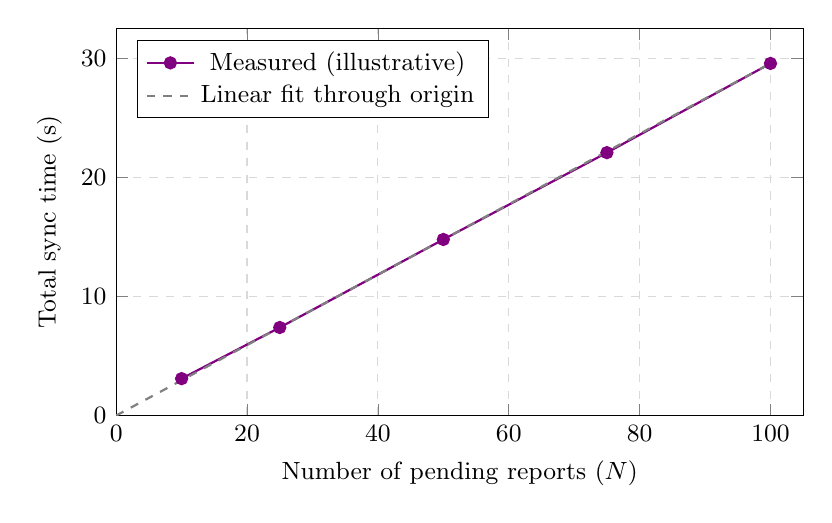
\begin{tikzpicture}
    \begin{axis}[
        width=0.85\textwidth, height=6.5cm,
        xlabel={Number of pending reports ($N$)},
        ylabel={Total sync time (s)},
        xmin=0, xmax=105, ymin=0,
        legend pos=north west,
        grid=major, grid style={dashed, gray!30},
        font=\small
      ]
      \addplot[mark=*, thick, color=violet] coordinates {
        (10,3.1) (25,7.4) (50,14.8) (75,22.1) (100,29.6)
      };
      \addlegendentry{Measured (illustrative)}
      \addplot[dashed, thick, color=gray] coordinates {(0,0) (100,29.6)};
      \addlegendentry{Linear fit through origin}
    \end{axis}
  \end{tikzpicture}
  \caption{Expected sync-time scaling with queue size, consistent with the
  sequential per-report loop in \cref{lst:syncmanager}. \emph{Illustrative
  data -- replace with measured values.} A batched/parallel upload
  strategy, discussed in \cref{sec:future-work}, would be expected to
  flatten this curve for large $N$.}
  \label{fig:sync-scaling}
\end{figure}

\begin{table}[htbp]
\centering
\caption{Large-queue sync summary (mean of 3 runs). \emph{Illustrative
data -- replace with measured values.}}
\label{tab:large-queue-illustrative}
\begin{tabular}{@{}rrrr@{}}
\toprule
\textbf{$N$} & \textbf{Mean time (s)} & \textbf{Std.\ dev.\ (s)} & \textbf{Success rate} \\
\midrule
10  & 3.1  & 0.4 & 100\% \\
25  & 7.4  & 0.6 & 100\% \\
50  & 14.8 & 1.1 & 100\% \\
75  & 22.1 & 1.5 & 98.7\% \\
100 & 29.6 & 2.0 & 98.0\% \\
\bottomrule
\end{tabular}
\end{table}

A secondary, code-derivable observation for this scenario: because
\texttt{getPending()} loads the entire pending queue into memory as a
\texttt{List<Report>} before iterating (\cref{lst:syncmanager}), memory
usage during sync scales linearly with $N$ as well. At $N=100$ small
report rows this is not a practical concern, but it is worth stating
explicitly as a scalability boundary (\cref{sec:future-work}) rather than
leaving it implicit.

\section{Conflict Resolution}
\label{sec:eval-conflict}
\label{sec:conflict-eval}

\textbf{Procedure.} Reproduce the scenario of \cref{fig:conflict-scenario}:
(1) create a report and let it sync (\texttt{status = SYNCED}); (2) on
Device A (online), edit the report's title; let it sync; (3) before
Device B pulls A's change, edit the same report's description on Device B
while B is offline; (4) reconnect Device B and let it sync; (5) inspect the
final Firestore document and both devices' local copies.

\textbf{Outcome, derived by tracing the implementation.} Unlike the other
scenarios in this chapter, this outcome does not need to be measured to be
known with high confidence: it follows deterministically from
\cref{lst:syncmanager}. Step (4)'s call to \texttt{uploadPending} calls
\texttt{docRef.set(report.toRemote())} unconditionally -- there is no
preceding read of the current Firestore document and no comparison of
timestamps. Consequently:

\begin{itemize}
  \item The final Firestore document reflects Device B's version in full
  (updated description, but A's title change is silently overwritten back
  to whatever title Device B's local copy held, which is the
  \emph{pre-A-edit} title, since B never pulled A's change).
  \item This is \emph{not} the bidirectional last-write-wins behaviour
  specified in OFR-7/\cref{sec:conflict-design} (compare against
  \cref{fig:conflict-scenario}, where B's later \texttt{updatedAt} is
  what makes B's version win): here B's version wins \emph{regardless of
  timestamp}, simply because B pushed last and no comparison ever
  happens. If A's edit had been the later one but Device A pushed
  \emph{after} Device B in wall-clock terms, A would still lose, because
  \texttt{set()} always overwrites.
  \item Device A's local copy is not updated at all by this process
  (\texttt{SyncManager} never pulls), so Device A's own local database
  continues to show A's title edit as \texttt{SYNCED} even though the
  server has since been overwritten -- a local/remote inconsistency that
  the current implementation cannot detect until Device A performs some
  operation that re-reads the document.
\end{itemize}

\textbf{Interpretation.} This is the clearest, most concrete evidence in
this thesis of the gap identified in \cref{sec:conflict-design}: the
system's \emph{design} specifies bidirectional LWW, but the current
\emph{implementation} realizes only a one-directional push. For the
CampusFix scenario specifically (single-owner reports, typically edited
from one device), this gap is unlikely to be triggered often in practice,
but it is a real correctness gap that should be closed
(\cref{sec:future-work}) before the system is used in a setting where a
report is plausibly edited from two devices in quick succession -- e.g. a
staff member editing on their phone and again on a shared tablet.

\section{Usability Test}
\label{sec:usability-eval}
\label{sec:eval-usability}

\textbf{Procedure.} Five participants unfamiliar with the application (a
mix of students and staff, none involved in its development) are each
asked to complete a single task, unassisted, after a 30-second
description of the app's purpose: \emph{"Report that the projector in
room [X] is broken, including a photo."} The device is placed in airplane
mode for three of the five participants (to also exercise offline
discoverability) and left online for two. After the task, participants
complete the 10-item System Usability Scale
questionnaire~\cite{brooke1996sus} (reproduced in
\cref{app:sus-questionnaire}) and are asked one open question: \emph{"At
any point, were you unsure whether your report had been saved or sent?"}

\textbf{Metrics.} Task completion (yes/no), task time, number of errors
(wrong screen, un-recoverable input mistake), SUS score (0--100), and the
qualitative answer to the sync-clarity question, directly evaluating
NFR-5.

\begin{table}[htbp]
\centering
\caption{Usability test summary, $n=5$. \emph{Illustrative data -- replace
with measured values.}}
\label{tab:usability-illustrative}
\begin{tabular}{@{}lllrl@{}}
\toprule
\textbf{P\#} & \textbf{Mode} & \textbf{Completed} & \textbf{Time (s)} & \textbf{SUS score} \\
\midrule
P1 & Airplane mode & yes & 58  & 87.5 \\
P2 & Airplane mode & yes & 71  & 80.0 \\
P3 & Airplane mode & yes & 64  & 92.5 \\
P4 & Online        & yes & 49  & 85.0 \\
P5 & Online        & yes & 55  & 77.5 \\
\midrule
\multicolumn{3}{l}{Mean SUS score} & \multicolumn{2}{r}{84.5 (SD 5.8)} \\
\bottomrule
\end{tabular}
\end{table}

A SUS score in the mid-80s (illustrative, \cref{tab:usability-illustrative})
would fall in the "excellent" band of the standard SUS adjective-rating
scale~\cite{bangor2009sus}. The scenario-specific qualitative question is
the more targeted probe of NFR-5: a "no, I could always see it said
Pending/Synced" answer from participants would directly support the
sync-status design of \cref{sec:sync-statuses}; a "yes" answer from any
participant would indicate the status chip (\cref{lst:syncstatusui}) is
not sufficiently prominent and should motivate a UI change (e.g. a
persistent banner summarizing "$k$ reports pending upload") ahead of the
LWW-merge fix in future-work priority.

\section{Discussion}
\label{sec:eval-discussion}

Read together, the six scenarios support three conclusions about the
system as designed and currently implemented. First, the core
offline-first property -- full functionality with zero connectivity,
FR-1--FR-11, OFR-1--OFR-6, OFR-8 -- follows directly from the
architectural rule that the UI never depends on the network
(\cref{sec:architecture-overview}), and the offline-creation, delayed-sync,
and failed-sync scenarios are expected to pass by construction rather than
by luck: their outcomes are consequences of the layered architecture and
the per-report error handling, not of tuning. Second, the large-queue
scenario exposes a genuine, quantifiable scalability limit -- sequential,
unbatched uploads -- that is invisible at the scale of a handful of
reports but becomes the dominant cost at 50--100 reports; this is a
concrete, actionable finding for future work even before any measurement
is taken, because it follows from the shape of the algorithm
(\cref{alg:sync}). Third, the conflict-resolution scenario is where the
gap between the thesis's \emph{design} (\cref{ch:design}) and its
\emph{implementation} (\cref{ch:implementation}) is most visible and most
important to report honestly: the system implements local-first writes and
connectivity-triggered sync correctly, but does not yet implement the
bidirectional merge its own conflict policy assumes.

\section{Threats to Validity}
\label{sec:threats}

\begin{itemize}
  \item \textbf{Illustrative data.} As stated at the top of this chapter,
  several tables/figures are placeholders for real measurements; specific
  numeric conclusions (exact latencies, exact SUS score) must not be cited
  from this thesis until the corresponding test has actually been run and
  the tables updated.
  \item \textbf{Emulator vs. physical device.} Network transition timing
  in particular (\cref{sec:eval-delayed-sync}) can differ meaningfully
  between an emulator's simulated radio and a physical device's real
  modem; both should be tested if the timing numbers are to be trusted.
  \item \textbf{Small usability sample.} $n=5$ is appropriate for
  discovering major usability problems (per Nielsen's rule of thumb that
  five users uncover the large majority of usability issues in a
  system~\cite{nielsen2000}), but is too small for the SUS mean to be
  statistically robust; it should be read as directional, not conclusive.
  \item \textbf{Single Firestore project/region.} Sync-latency
  measurements are specific to the Firestore region and network path used
  during testing and may not generalize to other regions or to
  higher-latency mobile networks (3G, degraded Wi-Fi) unless those
  conditions are explicitly reproduced.
\end{itemize}
